\documentclass[12pt]{article}
\usepackage[left=12mm,top=0.5in,bottom=5in]{geometry}
\usepackage[utf8]{inputenc} 
\usepackage[T2A]{fontenc} 
\usepackage{enumitem} 
\usepackage{graphicx} %зураг
\usepackage[mongolian]{babel}

\usepackage{anysize}
\marginsize{3cm}{1.5cm}{2cm}{2cm}

\begin{document}
	
	
	
\section     {Гарчиг}
               0.1 Оршил .....................................................
               
               1.1. ..........................................................
               
               1.2............................................................
               
               
               
               
               
               
               
               
               
               
               
               
               
               
               
               
               
               
\end{document}             
               
               
               
               
               
               
               
               
               
               
               
               
               
               
               
               
               
               
               
               
               
               
               
               
               
               
               
               
               
               
               
               
               
               
               
               
               
               
               
               
               
               
               
               
\section                            {ОРШИЛ}
	Сүүлийн үед мэдээллийн технологи асар хурдацтай хөгжиж байгаагаас байгууллгага, аж ахуйн нэгжийн үйл ажиллагааны хэв маяг ч өөрчлөгдөж байна. 
	Ийнхүү албан байгууллага, хувь хүн, үйлдвэрүүдийн үйл ажиллагаа компьютер буюу тооцоолон бодох машинтай салшгүй холбоотой болсон ба тэр дундаа хүний хийх ажлыг хөнгөвчлөх, ажлын бүтээмжийг өндөрсгөх зэрэг асуудал нь нэн чухлаар тавигдаж байгаа. 
	Өнөөгийн мэдээллийн зуун гэж нэрлэгдсэн энэ үед хэн мэдээлэл сайн олж чадаж байна тэр чинээгээрээ амжилт олж чадах болсон. Иймд аливаа байгууллагын үйл ажиллагааг зохион байгуулах, мэдээллийн урсгалыг тодорхой болгож, мэдээллийг хурдан дамжуулах шаардлага зайлшгүй тулгар ч байна. Иймд интернет болон компьютерийн тусламжтай Сургуулийн цахим хуудсийг ажиллуулах нь багш оюутнууд ажил хичээлээ явуулхад тулгарсан ямар нэг асуудлийг шийдхэд нэн чухал үүрэг гүйцэтгэх юм.
	Ижил төстэй програмын судалгаа
	Энэ хүү санал асуулгийн модул нь Facebook-ийн Poll гэх модулаас санаа авсан бөгөөд хувь хүний хоорондийн групп чат болон хуудасны үйл ажиллагааны талаарх хуудасны нийт бүх гишүүдээс санал авах санал хураах үүднээс ашигладаг.Тухайн гишүүдэд санал асуулгын талаарх дүн харагдах байдал нь өнгө болон  хувиар илэрхийлэгдэж харагдах ба хэрэглэгчид энгийн бөгөөд ойлгомжтой ашиглахад хялбар байна. 

\section  {Хэрэглэгчийн тухай мэдээлэл}
	Энэхүү модулийн хэрэглэгчид нь тухайн сургуулийн багш болон туслах багш бас оюутан юм. Хэрэглэгч нь ямар нэг үйл ажиллагаа болон тухайн системд байгаа гишүүдийн талаарх өөрсдийн санал хүсэлт болон санал асуулгийг авах зорилгоор чат болон тухайн хуудас хэрэглэгч өөрийн хуудсанд үүсгэж ашиглаж болно.
\section  {Хэрэглэгчийн үйл ажиллагааны онцлог}
       {Админ:} Админ нь уг системын хэрэглэгч бөгөөд ямар нэгэн үйл ажиллагааны талаарх мэдээллийг оруулж өгснөөр гишүүдийн хооронд санал асуулга явуулах зорилгоор энэ модулыг ашгилна.
   
   {Багш:} Энэ модулыг  өөрийн хуудсанд үүсгэж оюутнуудийн санал бодлийг сонсох хичээлийн талаарх санал хүсэлт судалгаа хийх зорилгоор ашиглаж болно. 
   
   {Оюутан:} Энэ модулыг мөн өөрийн хувийн чат болон сургуулийн групп чатанд санал хүсэлтээр хэлэлцүүлэг хийх болон бөөнөөр шийдвэрлэх асуудлийг  явуулж болно.
	
	\title{Сургуулийн онлайн системийн санал асуулга модул}
	\author{О.Сугараа}
	\section{Хэрэглэгчийн функциональ шаардлага}
\textit {Админ}
		\begin{itemize}[label=*, nosep]
		\item Нэвтрэх
		\item Мэдээллийг шинэчлэх 
		\item Санал асуулга үүсгэх
		\item Санал асуулга цэсыг сонгох
		\item Санал асуулга өгөх
		\item Санал асуулга харах
	\end{itemize}

\textit {Хэрэглэгч}
	\begin{itemize}[label=*, nosep]
		\item Нэвтэрсэн байх
		\item Санал асуулга сонгох
		\item Санал асуулга өгөх 
		\item Санал асуулга харах
	\end{itemize}
	
	\section{Хэрэглэгчийн функциональ бус шаардлага}
\begin{itemize}[label=*, nosep]
	\item Санал асуулга өгсөн байх 
	\item Нэг хэрэглэгч нэг саналыг нэг л бөглөх
\end{itemize}
	\begin{center}
	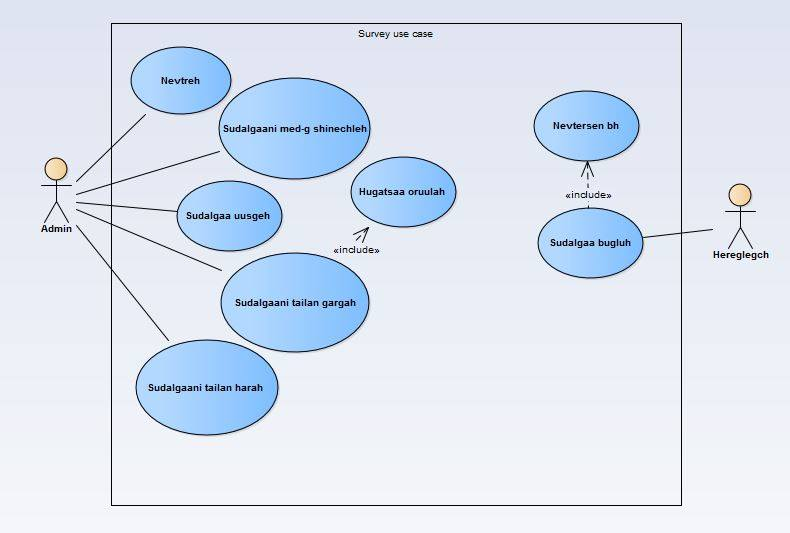
\includegraphics[scale=0.7]{survey.jpg}
\end{center}
\end{document}
